\documentclass[12pt]{article}
\usepackage[utf8]{inputenc}
\usepackage{amsmath, amssymb}
\usepackage{graphicx}
\usepackage{float}
\usepackage{booktabs}
\usepackage{geometry}
\usepackage{hyperref}
\usepackage{natbib}
\usepackage{caption}
\usepackage{tikz}
\usetikzlibrary{positioning,calc}

\geometry{margin=1in}

\title{Titanic Bayes Analysis}

% Define TikZ styles globally 
\tikzset{
	variable/.style={circle, draw, semithick, minimum size=1cm, inner sep=2pt},
	arrow/.style={->, semithick}
}

\begin{document}
	
	\maketitle
	
	\section{Titanic Causal Model}
	This project aims to estimate the effect of Age, Class, and Sex on the survival chance of the Titanic. 
	
	\subsection{Data description}
	The Titanic dataset is provided by the \texttt{causaldata} package and contains 2201 observations. 
	Variables include Age, Sex, Class, and Survival. 
	Age is binary: 1 = child, 2 = adult. 
	Sex is binary: 0 = woman, 1 = man. 
	Class has 4 categories (1–4). 
	Survival is binary: 0 = not survived, 1 = survived. 
	
	\section{Causal Models}
	The first causal model that aims to determine the direct effect of age on the survival chance is the following:
	
\begin{figure}[H]
	\centering
		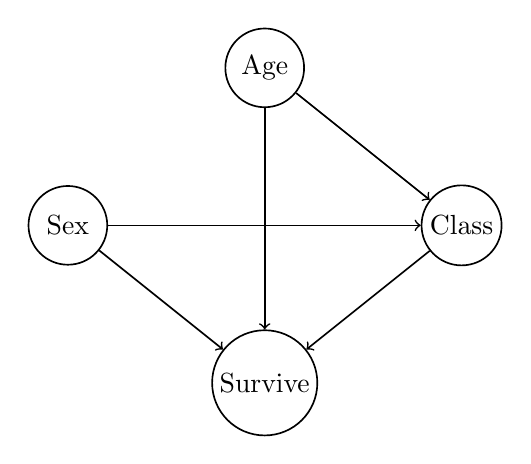
\begin{tikzpicture}
			% plain node definitions 
			\node[circle,draw,semithick,minimum size=1cm,inner sep=2pt] (age) {Age};
			\node[circle,draw,semithick,minimum size=1cm,inner sep=2pt] (sex) at (-2.5,-2) {Sex};
			\node[circle,draw,semithick,minimum size=1cm,inner sep=2pt] (class) at ( 2.5,-2) {Class};
			\node[circle,draw,semithick,minimum size=1cm,inner sep=2pt] (survive) at (0,-4) {Survive};
			
			% arrows
			\draw[->,semithick] (age) -- (class);
			\draw[->,semithick] (age) -- (survive);
			\draw[->,semithick] (sex) -- (class);
			\draw[->,semithick] (sex) -- (survive);
			\draw[->,semithick] (class) -- (survive);
		\end{tikzpicture}
	\caption{Causal Model to estimate the direct effect of Age on Survival chance}
	\label{fig:titanic_dag}
\end{figure}


Biasing paths are open.
Minimal sufficient adjustment sets for estimating the direct effect of Age on Survive include stratification by Class and Sex\\


The second Causal Model aims to determine the direct effect of Class on Survival in this case the minimal adjustment sets for estimating the direct effect of Class in Survival include stratification by Age and Sex\\


The third Causal Model aims to determine the direct effect of Sex on Survival and the minimal adjustment set is stratification by Class and Age\\

\section{Statistical Model}

\end{document}

